\documentclass[preview]{standalone}
\usepackage{ctex}

%graphics
\usepackage{xcolor}
\usepackage{tikz}
\usetikzlibrary{shapes.geometric, shapes.multipart, arrows, calc, through,intersections}
\usepackage[caption=false,font=footnotesize]{subfig}

\colorlet{dot-color}{black!80}
\tikzset{
    pics/cell/.style = {
        code = {%
        \coordinate (-center) at (0,0);
        
        \fill +(-0.495,-0.495) coordinate(-sw) 
           -- +(-0.495, 0.495) coordinate(-nw)
           -- +( 0.495, 0.495) coordinate(-ne)
           -- +( 0.495,-0.495) coordinate(-se)
           -- cycle;
        \coordinate (-swo) at ($ (-center)!0.5!(-sw) $);
        \coordinate (-nwo) at ($ (-center)!0.5!(-nw) $);
        \coordinate (-neo) at ($ (-center)!0.5!(-ne) $);
        \coordinate (-seo) at ($ (-center)!0.5!(-se) $);
        
        \coordinate (-south) at ($ (-sw)!.5!(-se) $);
        \coordinate (-north) at ($ (-nw)!.5!(-ne) $);
        \coordinate (-west)  at ($ (-sw)!.5!(-nw) $);
        \coordinate (-east)  at ($ (-se)!.5!(-ne) $);
        
        \fill[white] (-swo) let \p1=($ (-center)!.5!(-swo) $) in circle ({veclen(\x1,\y1)});
        \fill[white] (-nwo) let \p1=($ (-center)!.5!(-nwo) $) in circle ({veclen(\x1,\y1)});
        \fill[white] (-neo) let \p1=($ (-center)!.5!(-neo) $) in circle ({veclen(\x1,\y1)});
        \fill[white] (-seo) let \p1=($ (-center)!.5!(-seo) $) in circle ({veclen(\x1,\y1)});
        
        \ifnum#1=1\relax
            \fill[dot-color] (-swo) let \p1=($ (-center)!.32!(-swo) $) in circle ({veclen(\x1,\y1)});
            \fill[dot-color] (-neo) let \p1=($ (-center)!.32!(-neo) $) in circle ({veclen(\x1,\y1)});
        \else
            \ifnum#1=-1\relax
                \fill[dot-color] (-nwo) let \p1=($ (-center)!.32!(-nwo) $) in circle ({veclen(\x1,\y1)});
                \fill[dot-color] (-seo) let \p1=($ (-center)!.32!(-seo) $) in circle ({veclen(\x1,\y1)});
            \else
                \fill[dot-color] (-swo) let \p1=($ (-center)!.22!(-swo) $) in circle ({veclen(\x1,\y1)});
                \fill[dot-color] (-nwo) let \p1=($ (-center)!.22!(-nwo) $) in circle ({veclen(\x1,\y1)});
                \fill[dot-color] (-neo) let \p1=($ (-center)!.22!(-neo) $) in circle ({veclen(\x1,\y1)});
                \fill[dot-color] (-seo) let \p1=($ (-center)!.22!(-seo) $) in circle ({veclen(\x1,\y1)});
            \fi
        \fi
        }
    },
    pics/cell/.default={0},
    pics/maj/.style = {
        code = {%
        \coordinate  (P0) at (0,-1);
        
        \draw (P0) -- ++(45:1cm) coordinate (P1) -- ++(0,1cm) coordinate (P2) -- ($(P0)!(P2)!(0,5cm)$) coordinate (P3) -- ($(P3)!-1!(P2)$) coordinate (P4) -- ++(0, -1cm) coordinate (P5) -- cycle;
 
        \coordinate (-south) at (P0);
        \coordinate (-north) at (P3);
        \coordinate (-north east) at (P2);
        \coordinate (-north west) at (P4);
        \coordinate (-east) at ($(P1)!.5!(P2)$);
        \coordinate (-west) at ($(P4)!.5!(P5)$);
        \coordinate (-center) at ($(P3)!.5!(P0)$);
        
        \ifnum#1>0\relax
            \node at (0,0) {MV#1};
        \fi
        }
    },
    pics/maj/.default={0},
    pics/inv/.style = {
        code = {%
            \coordinate (P0) at (0,-1);
            
            \draw (P0) -- ++(65:1cm)  coordinate (P1) -- ($(P0)!(P1)!(0,5cm)$) coordinate (P2) -- ($(P2)!-1!(P1)$) coordinate (P3) -- (P0);
            
            \coordinate (circ_o) at ($(P0)-(0,0.1cm)$);
            
            \draw (circ_o) circle[radius=0.1cm];
            
            \coordinate (-input)  at (P2);
            \coordinate (-output) at ($(P0)-(0,0.2cm)$);
        }
    },
    pics/inv/.default={0},
}
% \definecolor{clock0}{HTML}{86E291}
% \definecolor{clock1}{HTML}{FFA5FA}
% \definecolor{clock2}{HTML}{00C8BC}
% \definecolor{clock3}{HTML}{F2F2F2}
% \definecolor{input}{HTML}{008DC8}
% \definecolor{output}{HTML}{E28686}
% \definecolor{fixed}{HTML}{000000}

\definecolor{clock0}{RGB}{89,89,91}
\definecolor{clock1}{RGB}{129,130,132}
\definecolor{clock2}{RGB}{210,210,212}
\definecolor{clock3}{RGB}{168,169,173}
\definecolor{input}{RGB}{230,230,230}
\definecolor{output}{RGB}{40,40,40}
\definecolor{fixed}{HTML}{000000}


\begin{document}

\begin{figure}[!t]
\centering
\subfloat[电路原理图]{
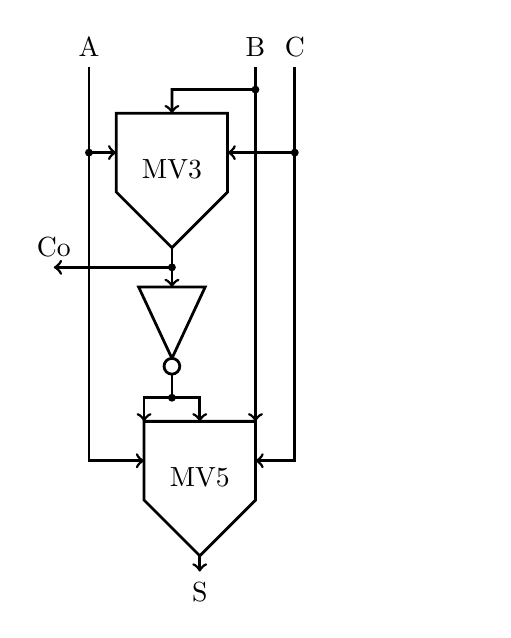
\begin{tikzpicture}[transform shape,line width=1pt]
\pic (m5)at (0,0) {maj=5};
\coordinate (m5anchor) at ($(m5-north)!0.5!(m5-north west)$);
\pic (i)  at ($(m5anchor)+(0,1.8cm)$) {inv};
\pic (m3) at ($(i-input)+(0,1.5cm)$) {maj=3};

\draw[<-,name path=AM] ($(m5-west)$) -- ($(m5-west)+(-0.7cm,0)$) -- ++(0,5cm) coordinate(A);
\node[above]at (A){A};
\path[name path=AB] (A) -- ++(5cm,0);
\path[name path=BM] (m5-north east) -- ++(0, 5cm);
\path [name intersections={of=AB and BM,by=B}];
\draw[<-] (m5-north east) -- (B) node[above]{B};
\coordinate (C) at ($(B)+(0.5cm,0)$);
\draw[<-,name path=CM] (m5-east) -| (C) node[above]{C};

\draw[->] (m3-south) -- (i-input);
\coordinate (m3i) at ($(m3-south)!.5!(i-input)$);
\fill(m3i) circle [radius=0.05cm];
\coordinate (im5) at ($(i-output)!.5!($(m5-north east)!(i-output)!(m5-north west)$)$);
\draw (i-output) -- (im5);
\fill(im5) circle [radius=0.05cm];
\draw[->] (im5) -| (m5-north west);
\draw[->] (im5) -| (m5-north);

\draw[<-] (m3-north) -- ++ (0,0.3cm) coordinate (m3b) -- ($(B)!(m3b)!(m5-north east)$) coordinate (bp1);
\fill(bp1) circle [radius=0.05cm];
\draw[<-] (m3-west) -- ($(A)!(m3-west)!($(A)-(0,5cm)$)$) coordinate (ap1);
\fill(ap1) circle [radius=0.05cm];
\draw[<-] (m3-east) -- ($(C)!(m3-east)!($(C)-(0,5cm)$)$) coordinate (cp1);
\fill(cp1) circle [radius=0.05cm];
\draw[->] (m3i) -- ++(-1.5cm,0) node[above]{Co};
\draw[->] (m5-south) -- ++(0,-0.2cm) node[below]{S};
\end{tikzpicture}
}
\subfloat[QCA版图]{
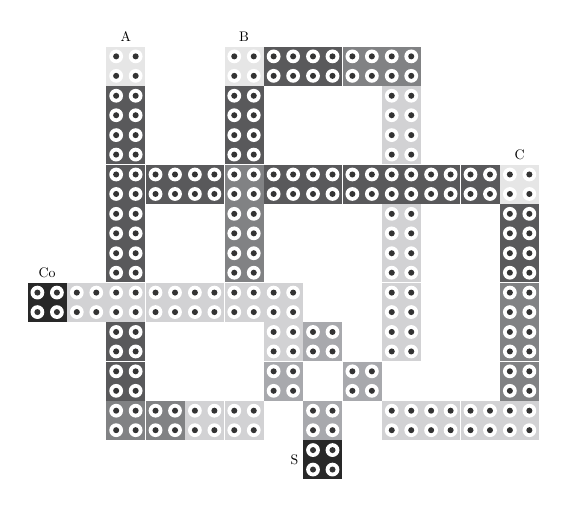
\begin{tikzpicture}[scale=0.5,transform shape]

\pic(Co)[output] at (0,0) {cell};
\node[above] at (Co-north) {Co};

\pic[clock2] at (1,0) {cell};

\pic(A)[input] at (2,6) {cell};
\node[above] at (A-north) {A};
\pic[clock0] at (2,5) {cell};
\pic[clock0] at (2,4) {cell};
\pic[clock0] at (2,3) {cell};
\pic[clock0] at (2,2) {cell};
\pic[clock0] at (2,1) {cell};
\pic[clock2] at (2,0) {cell};
\pic[clock0] at (2,-1) {cell};
\pic[clock0] at (2,-2) {cell};
\pic[clock1] at (2,-3) {cell};

\pic[clock0] at (3,3) {cell};
\pic[clock2] at (3,0) {cell};
\pic[clock1] at (3,-3) {cell};

\pic[clock0] at (4,3) {cell};
\pic[clock2] at (4,0) {cell};
\pic[clock2] at (4,-3) {cell};

\pic(B)[input] at (5,6){cell};
\node[above] at (B-north) {B};
\pic[clock0] at (5,5) {cell};
\pic[clock0] at (5,4) {cell};
\pic[clock1] at (5,3) {cell};
\pic[clock1] at (5,2) {cell};
\pic[clock1] at (5,1) {cell};
\pic[clock2] at (5,0) {cell};
\pic[clock2] at (5,-3) {cell};

\pic[clock0] at (6,6) {cell};
\pic[clock0] at (6,3) {cell};
\pic[clock2] at (6,0) {cell};
\pic[clock2] at (6,-1) {cell};
\pic[clock3] at (6,-2) {cell};

\pic[clock0] at (7,6) {cell};
\pic[clock0] at (7,3) {cell};
\pic[clock3] at (7,-1) {cell};
\pic[clock3] at (7,-3) {cell};
\pic(S)[output] at (7,-4) {cell};
\node[left] at (S-west) {S};

\pic[clock1] at (8,6) {cell};
\pic[clock0] at (8,3) {cell};
\pic[clock3] at (8,-2) {cell};

\pic[clock1] at (9,6) {cell};
\pic[clock2] at (9,5) {cell};
\pic[clock2] at (9,4) {cell};
\pic[clock2] at (9,3) {cell};
\pic[clock0] at (9,3) {cell};
\pic[clock2] at (9,2) {cell};
\pic[clock2] at (9,1) {cell};
\pic[clock2] at (9,0) {cell};
\pic[clock2] at (9,-1) {cell};
\pic[clock2] at (9,-3) {cell};


\pic[clock0] at (10,3) {cell};
\pic[clock2] at (10,-3) {cell};

\pic[clock0] at (11,3) {cell};
\pic[clock2] at (11,-3) {cell};

\pic(C)[input] at (12,3) {cell};
\node[above] at (C-north) {C};
\pic[clock0] at (12,2) {cell};
\pic[clock0] at (12,1) {cell};
\pic[clock1] at (12,0) {cell};
\pic[clock1] at (12,-1) {cell};
\pic[clock1] at (12,-2) {cell};
\pic[clock2] at (12,-3) {cell};

\end{tikzpicture}
}
\end{figure}

\end{document}
